\newpage

  \noindent\textbf{\large 4. Построение преобразователей угол-код на синусно-косинусных решающих устройствах}

\refstepcounter{chapter}
\addcontentsline{toc}{chapter}{4. ПОСТРОЕНИЕ  ПРЕОБРАЗОВАТЕЛЕЙ УГОЛ-КОД НА СИНУСНО-КОСИНУСНЫХ РЕШАЮЩИХ УСТРОЙСТВАХ}


\section{Классические схемы}

Существует широкий класс схем преобразоваталей угол-код.
В \cite{Vulvet} описан целый ряд различных методов построения преобразователей угол-код: 

\begin{itemize}
  \item контактные кодирующие преобразователи;
  \item магниторезистивные преобразователи;
  \item аналоговые схемы с использованием RLC-цепей для формирования сигналов;
  \item трансформаторные системы, основанные на взаимной индукции.
\end{itemize}

Однако такие решения обладают некоторыми существенными недостатками в современных условиях.
\begin{itemize}
  \item \textbf{Считывание}: Использование моточных изделий (трансформаторов, катушек) увеличивает массу и габариты устройств.
  \item \textbf{Устаревание}: В связи с совершенствованием схем контроллеров, появляются возможности для более оптимальных.
  \item \textbf{Сложность настройки}: усложняется производство и снижается надежность, ввиду необходимости индивидуальной ручной подстройки аналоговых ком­
понентов.
  \item \textbf{Низкая совместимость} с цифровыми системами управления.
\end{itemize}

Развитие микропроцессорной техники и миниатюризация контроллеров привели к переходу на компактные и энергоэффективные решения
Современные преобразователи исключают громоздкие аналоговые компоненты, заменяя их программируемыми схемами


\section{Современные подходы}

В современных системах преобразования углового положения в цифровой код доминируют два технологических подхода, обеспечивающих оптимизацию массогабаритных характеристик без снижения точности позиционирования:
\begin{enumerate}
    \item цифровые преобразователи на базе микроконтроллеров,
    \item гибридные схемы с интегрированными микросхемами.
\end{enumerate}

\textbf{Ключевые особенности цифровых преобразователей:}
\begin{itemize}
    \item применение АЦП и алгоритмов цифровой обработки сигналов (ЦОС);
    \item отсутствие моточных компонентов, обеспечивающее снижение массы конструкции на 30-40\%;
    \item достижение точности преобразования $\pm 0.1^\circ$ за счёт программной компенсации систематических погрешностей.
\end{itemize}

\textbf{Ключевые особенности гибридных решений:}
\begin{itemize}
    \item комбинирование аналоговых синусно-косинусных генераторов с цифровыми интерфейсами (SPI, I$^2$C);
    \item использование специализированных интегральных схем (например, AD2S1210, К1310НМ025 \cite{Spec}), минимизирующее количество внешних компонентов;
    \item обеспечение разрешения до 16 бит при сохранении минимальных габаритов.
\end{itemize}

\subsection{Преимущества современных подходов в сравнении с аналоговыми решениями}
\begin{itemize}
    \item \textbf{Миниатюризация}: Отказ от трансформаторов снижает объем устройства в 2–3 раза.
    \item \textbf{Повышенная надежность}: Цифровая обработка исключает дрейф параметров аналоговых компонентов.
    \item \textbf{Совместимость}: Интеграция с промышленными сетями (CAN, Ethernet) упрощает внедрение.
\end{itemize}

Таким образом, классические схемы, описанные в ранних работах, уступают современным цифровым и гибридным решениям по ключевым параметрам. 
Переход на микроконтроллерные системы и специализированные ИС позволяет достичь высокой точности при минимальных массогабаритных показателях, 
что особенно актуально для аэрокосмических и робототехнических применений.

В части цифровой обработки сигналов датчиков в цифровых преобразователях выделяют две основные схемы:
\begin{itemize}
    \item метод прямого преобразования,
    \item следящее преобразование
\end{itemize}
Рассмотрим их подробнее.

\subsection{Метод прямого преобразования}
\subsubsection{Принцип работы}
Метод прямого преобразования \cite{Armenski} основан на вычислении угла поворота через арктангенс отношения синусоидального (\(U_{\sin}\)) и косинусоидального (\(U_{\cos}\)) сигналов:
\begin{equation}
\theta = \arctan\left(\frac{U_{\sin}}{U_{\cos}}\right).
\end{equation}


Для реализации метода используются два АЦП, оцифровывающих сигналы с датчика. Разрядность АЦП напрямую влияет на точность: 
\begin{equation}
\Delta\theta = \frac{360^\circ}{2^N},
\end{equation}
где \(N\) — разрядность АЦП.

Например, для \(N = 12\) бит:
\begin{equation}
\Delta\theta = \frac{360^\circ}{4096} \approx 0.088^\circ.
\end{equation}

\subsubsection{Проблемы метода}
Метод прямого преобразования угла в код через вычисление арктангенса отношения синусоидального и косинусоидального сигналов сталкивается со следующими ограничениями:
\begin{itemize}
    \item \textbf{Зависимость от качества сигналов} \\
    Шумы, нелинейности и фазовые сдвиги в сигналах \( U_{\sin} \) и \( U_{\cos} \) приводят к систематическим ошибкам. Например, асимметрия амплитуд вызывает погрешность:
    \begin{equation}
    \Delta\theta = \arctan\left(\frac{U_{\sin} + \delta}{U_{\cos}}\right) - \arctan\left(\frac{U_{\sin}}{U_{\cos}}\right),
    \end{equation}
    где \(\delta\) — отклонение амплитуды.

    \item \textbf{Высокие требования к АЦП} \\
    Для точности \(\Delta\theta < 0.1^\circ\) требуется разрядность АЦП не менее 16 бит:
    \begin{equation}
    N = \log_2\left(\frac{360^\circ}{\Delta\theta}\right) \approx 16.
    \end{equation}

    \item \textbf{Нелинейности и калибровка} \\
    Отклонения от идеальной синусоиды требуют использования таблиц поправок, увеличивая сложность алгоритма. 
    Появляющеся в процессе работы нелинейности скомпенсированы не будут.

    \item \textbf{Чувствительность к внешним факторам} \\
    Температурный дрейф компонентов (например, АЦП) снижает стабильность:
    \begin{equation}
    \Delta\theta_{\text{дрейф}} = \alpha \cdot \Delta T,
    \end{equation}
    где \(\alpha\) — температурный коэффициент, \(\Delta T\) — перепад температуры.

    \item \textbf{Проблемы при малых сигналах} \\
    При \(\theta \to 0^\circ\) или \(90^\circ\) отношение \( U_{\sin}/U_{\cos} \) стремится к \(0\) или \(\infty\), увеличивая погрешность из-за дискретизации.
\end{itemize}

Таким образом метод прямого преобразования подходит для статических систем с умеренными требованиями к точности. 
В динамических или высокоточных приложениях предпочтительны преобразователи с обратной связью, компенсирующие перечисленные недостатки.

\subsection{Следящие преобразователи}

\textbf{Принцип работы}
Следящие преобразователи (СП) используют замкнутый контур управления для минимизации рассогласования между текущим углом и заданным значением. 
Сигналы \(U_{\sin}\) и \(U_{\cos}\) сравниваются с опорными, а ошибка подается на корректирующий элемент (например, двигатель) \cite{Anufriev2014} \cite{Safronov}.

\textbf{Структура СП}
\begin{itemize}
    \item \textbf{Фазовый детектор}: Вычисляет разность фаз между входными и опорными сигналами.
    \item \textbf{Интегратор}: Формирует управляющий сигнал для исполнительного механизма.
    \item \textbf{Обратная связь}: Обеспечивает точность \(\pm0.01^\circ\) за счет коррекции в реальном времени.
\end{itemize}

\textbf{Современные подходы к реализации}

Следящие преобразователи обеспечивают прецизионное управление в динамических системах, но требуют сложной настройки.
Поэтому чаще всего для обсчета используются программируемые логические интергальные схемы (ПЛИС) или микроконтроллеры \cite{MilandrSKVT}.

\section{Формирование технического задания на проектируемое устройство}

Конфигурация разрабатываемой измерительной системы включает два синусно-косинусных вращающихся трансформатора (СКВТ). 
Применение специализированных интегральных схем (ИС) для обработки сигналов СКВТ потребовало бы использования двух микросхем (по одной на каждый датчик). 

Вследствие экономической нецелесообразности применения указанных ИС (высокая стоимость компонентов) и ограниченной доступности компонентной базы 
на рынке поставок, было обосновано решение о разработке специализированного печатного узла. В качестве базовой вычислительной платформы выбран микроконтроллер 
семейства STM32 с ядром ARM Cortex-M7 (серия F7).

На основании проведенного анализа элементной базы, моделирования и расчетов ключевых параметров системы было сформировано техническое задание на устройство. 
Основной целью разработки ТЗ является обеспечение следующих требований:
\begin{itemize}
    \item совместимость с интерфейсом СКВТ, 
    \item обработка сигналов двух датчиков в реальном времени,
    \item соответствие точностным характеристикам системы,
    \item надежность эксплуатации.
\end{itemize}

\subsection{Назначение и состав изделия}
Разрабатываемый печатный узел представляет собой блок аналого-цифрового преобразователя сигналов вращающегося трансформатора (АЦПВТ), 
предназначенный для измерения углового положения в одной степени свободы антенной системы. Функционирование устройства реализовано по двухотсчетной 
схеме с передаточным отношением редуктора между датчиками грубого и точного отсчета 1:36.

\subsection{Основные технические требования}

    На рис.~\ref{FuncBlocks} представлена структурная схема устройства. 
    \begin{itemize}
    \item Через разъём СНП-59  необходимо обеспечить подключение к датчикам углового положения и концевым выключателям приборного редуктора. 

    \item Внутренняя структура блока должна включать схемы обработки сигналов вращающихся трансформаторов и концевых выключателей. 

    \item Преобразованные сигналы должны передаваться на ведущее устройство посредством микроконтроллерной платформы с интегрированным приёмопередатчиком RS-422.
    
    \item Для обеспечения функциональной безопасности должен быть предусмотрен дополнительный разъём, подключенный параллельно концевым выключателям приборного редуктора. 
    Данное решение позволяет реализовать цепи аварийного отключения посредством последовательного включения нормально-заикнутых концевых выключателей 
    в цепь питания главного контактора шкафа электропривода.


    \item В печатном узле необходимо обеспечить совместимость с вращающимися трансформаторами типа ЛИР-ДР158А.

    \item Для информационного обмена используется последовательный синхронный интерфейс SSI \cite{SSI} со следующими параметрами:
        \begin{table}[h]
        \centering
        \begin{tabular}{|l|l|}
        \hline
        Параметр & Значение \\ \hline
        Тактовая частота Clock & 100 кГц \\ \hline
        Кодирование выходного сигнала & Код Грея \\ \hline
        Формат данных & 18-битное MSB-first представление угла \\ \hline
        \end{tabular}
        \caption{Параметры интерфейса SSI}
        \label{tab:ssi-params}
        \end{table}
    % \begin{itemize}
    %     \item Тактовая частота сигнала синхронизации (Clock): 100 кГц
    %     \item Кодирование выходной телеграммы: код Грея
    %     \item Формат данных: 18-битное представление углового положения (MSB-first)
    % \end{itemize}
\end{itemize}


 
\FloatBarrier
\subsection{Конструктивные требования}
Конструктивное исполнение блока АЦПВТ должно представлять собой сменный картридж, обеспечивающий герметичность соединения при установке в корпус приборного 
редуктора. Компоненты устройства размещаются на единой печатной плате, 
геометрические параметры которой определяются эскизами корпуса (рис. \ref{Corp1}, \ref{Corp2}).

\begin{figure}[htbp]
    \centering
    \begin{minipage}{0.48\linewidth}% ширина первой колонки
       \centering
        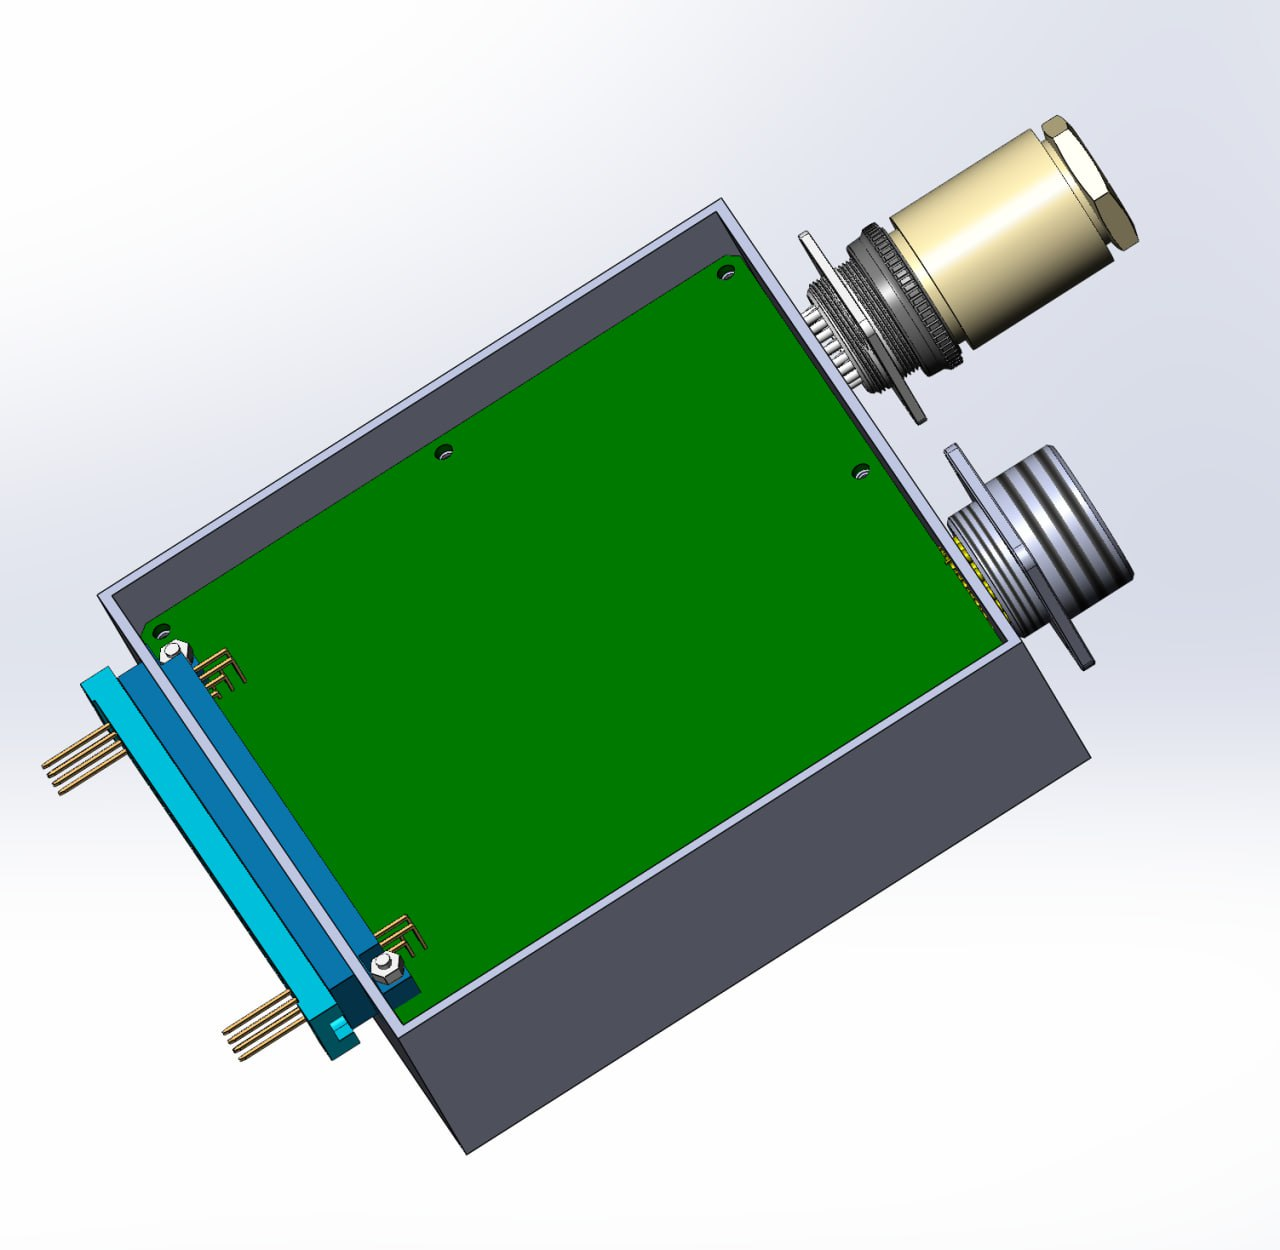
\includegraphics[width=\linewidth]{Corp1.jpg}
        \caption{Конструкция корпуса блока (вид А)}
        \label{Corp1}
    \end{minipage}\hfill% добавляем горизонтальное заполнение между изображениями
    \begin{minipage}{0.48\linewidth}% ширина второй колонки
       \centering
        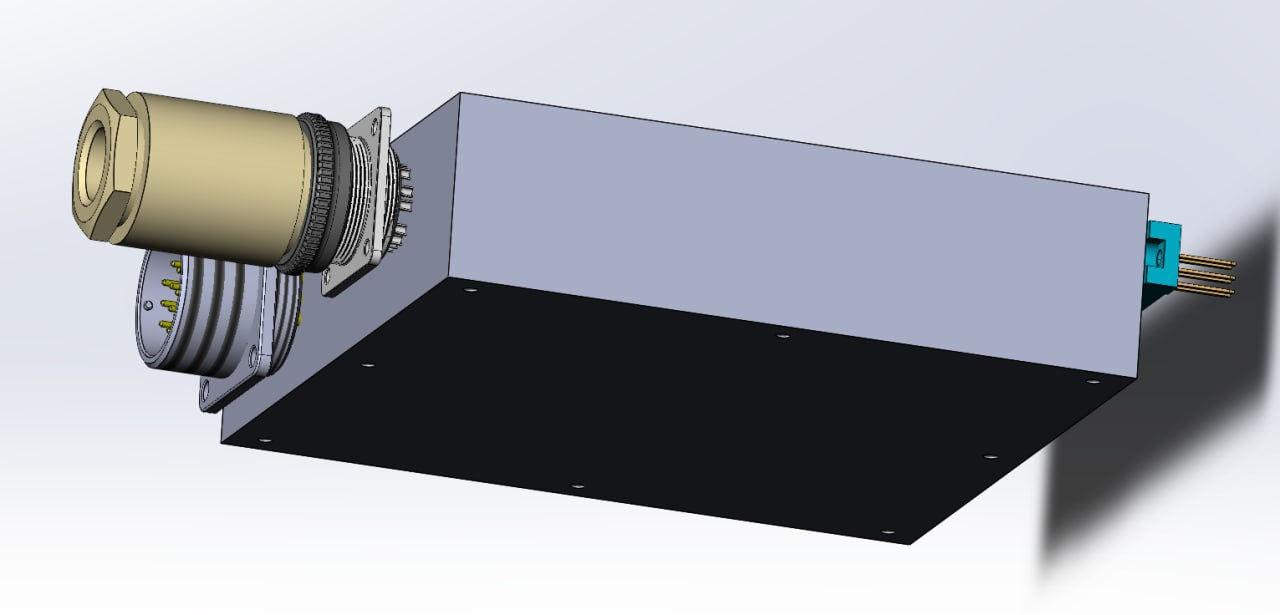
\includegraphics[width=\linewidth]{Corp2.jpg}
        \caption{Конструкция корпуса блока (вид Б)}
        \label{Corp2}
    \end{minipage}
\end{figure}


\FloatBarrier
\subsection{Требования по устойчивости к внешним воздействиям}
К устройству предъявляются повышенные требования по стойкости к климатическим воздействиям:
\begin{itemize}
    \item рабочий температурный диапазон: от $\text{минус} 40^\circ$C до $ 60^\circ$C;
    \item предельные температуры эксплуатации: от $\text{минус}60^\circ$C до $70^\circ$C;
    \item относительная влажность: до 95\% при $30^\circ$C;
    \item стойкость к конденсату влаги: при $\text{минус}25^\circ$C в течение 2 часов.
\end{itemize}

\FloatBarrier
\section{Конструкция печатного узла}

В результате проектирования, проведенного инженерами компании, изготовлен печатный узел блока аналого-цифрового преобразователя сигналов вращающегося трансформатора (АЦПВТ). 
Для генерации возбуждающего синусоидального сигнала применен внешний цифро-аналоговый преобразователь (ЦАП)\cite{DAC} с последующим каскадом усиления 
на полевых транзисторах (схема на стр. ~\pageref{DAC}). Данное решение обеспечивает преобразование выходного сигнала ЦАП (0-3,3 В) в требуемый для датчиков ЛИР-ДР158А диапазон ±7 В. 
Цифровой интерфейс ЦАП подключен к выделенному порту микроконтроллера для оптимизации управления. 

Обработка сигналов двух датчиков реализована на базе четырех внешних аналого-цифровых преобразователях (АЦП) \cite{ADC}, каждый из которых подключен к 
отдельному порту ввода-вывода (схема на стр. ~\pageref{ADC}).

% \begin{figure}[!h]
%   \centering 
%   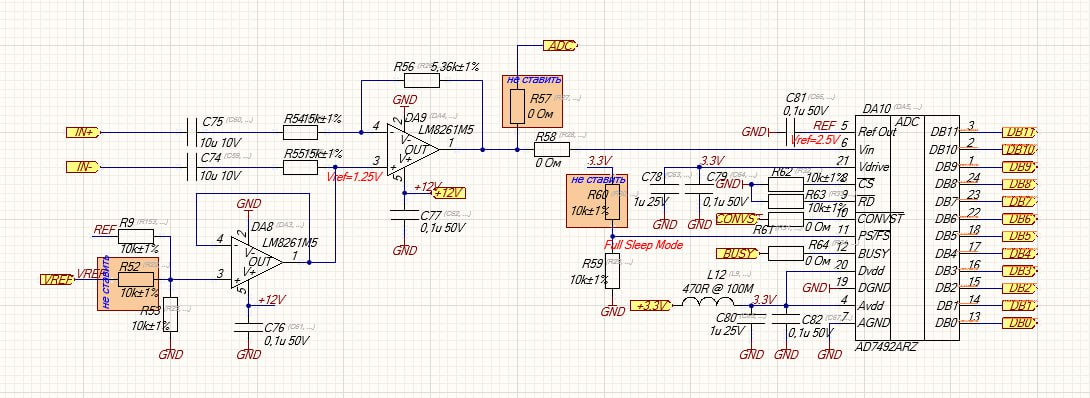
\includegraphics[width=\textwidth]{АЦП1.jpg} 
%   \caption{Схема включения АЦП}
%   \label{ADC}
% \end{figure}

% \begin{figure}[!h]
%   \centering
%   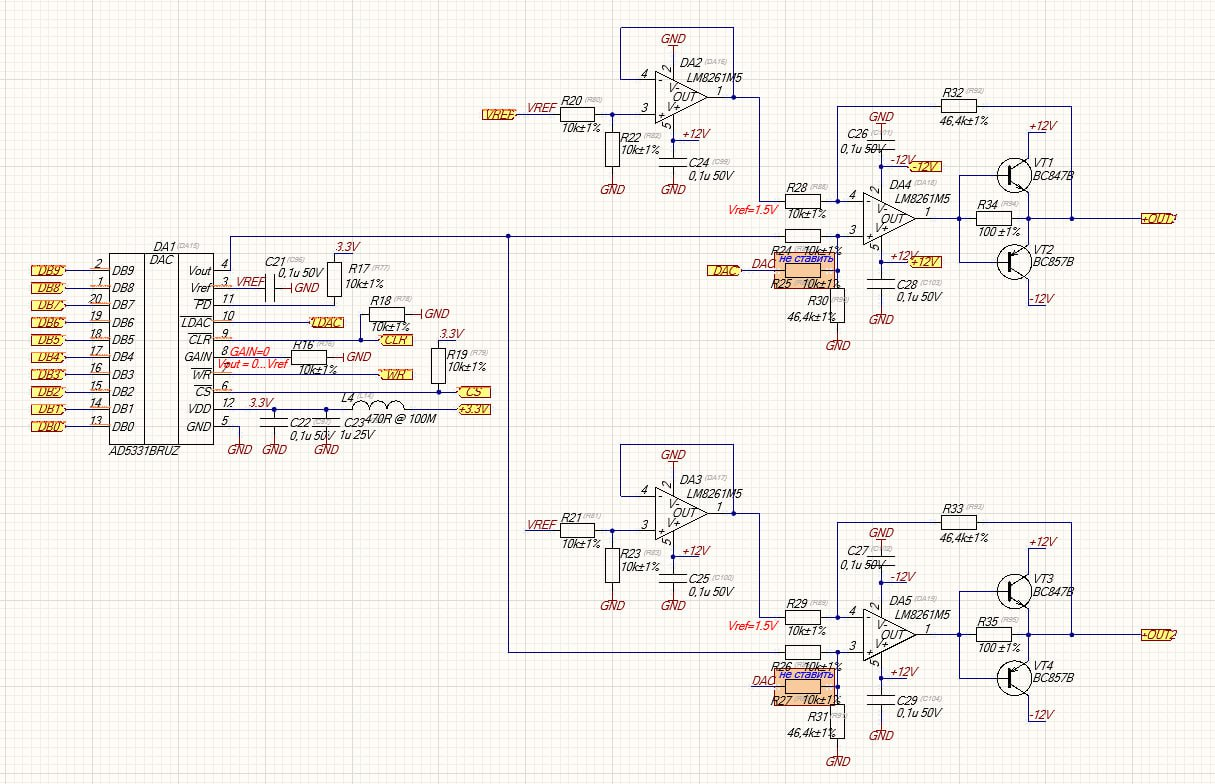
\includegraphics[width=\textwidth]{ЦАП1.jpg} 
%   \caption{Схема включения ЦАП}
%   \label{DAC}
% \end{figure}

\FloatBarrier

\section{Управляющие сигналы}
Для обеспечения временной синхронизации управляющих сигналов применена схема каскадного включения аппаратных таймеров по принципу 
"ведущий-ведомый" (рис. \ref{Timers}). 

Мастер-таймер TIM4 инициирует синхронный запуск подчиненных таймеров TIM3 и TIM9. 
Таймер TIM3 активирует передачу данных в ЦАП через контроллер прямого доступа к памяти (DMA). 
После завершения передачи TIM3 в режиме однократного импульса (one-pulse mode) формирует сигнал записи (Write Gen) в регистр ЦАП. 

Таймер TIM9 обеспечивает программируемую задержку для сигнала запуска преобразования АЦП (Conversion start). 
Данное решение позволяет выполнять выборку сигнала с датчика в точке максимальной амплитуды, что повышает точность измерений за счет полного 
использования динамического диапазона.

Считывание данных с параллельных интерфейсов АЦП осуществляется через DMA по прерыванию от спадающего фронта сигнала Busy. 
Поскольку сигнал Busy объединен по схеме логического "ИЛИ" для всех четырех каналов АЦП, чтение результатов преобразования происходит 
синхронно после завершения измерения последним преобразователем.

Применение аппаратных модулей синхронизации позволило достичь высокой временной точности (порядка 10 нс) и минимальной загрузки центрального процессора. 
Высвобожденные вычислительные ресурсы используются для:
\begin{itemize}
    \item реализации алгоритмов вычисления углового положения,
    \item обработки сигналов концевых выключателей,
    \item организации сетевого взаимодействия через интерфейс CAN.
\end{itemize}

\begin{figure}[!h]
  \centering
  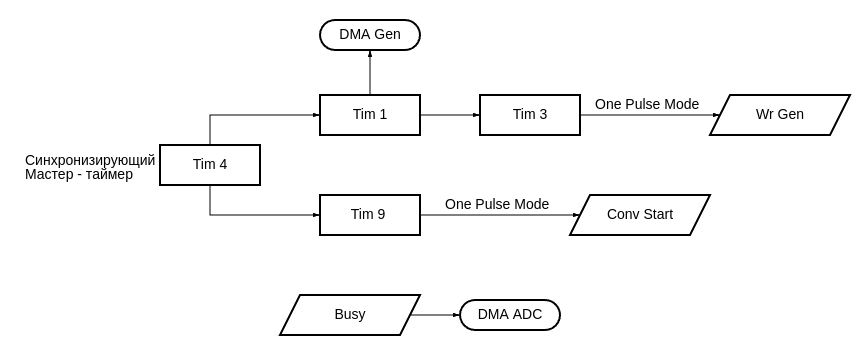
\includegraphics[width=0.95\textwidth]{TimersScheme1.png} 
  \caption{Схема синхронизации таймеров}
  \label{Timers}
\end{figure}

\textbf{картинка Форма возбуждающего сигнала на выходе ЦАП}
% \begin{figure}[!h]
%   \centering
%   \includegraphics[width=0.8\textwidth]{sine_wave.png} 
%   \caption{Форма возбуждающего сигнала на выходе ЦАП}
%   \label{SineWave}
% \end{figure}

\newpage
\section{Разработка следящего алгоритма}
После верфикации аппаратного управления работой микросхем и получения данных с АЦП, возникла задача реализации алгоритма вычисления углового положения. 
В ходе исследования методов обработки сигналов синусно-косинусных вращающихся трансформаторов (СКВТ) ЛИР-ДР158А был выбран метод следящего преобразования. 
Данный подход обеспечивает:
\begin{itemize}
    \item минимизацию систематических погрешностей,
    \item повышение разрешающей способности до 19 бит,
    \item компенсацию фазовых и скоростных рассогласований через контур обратной связи.
\end{itemize}

\subsection{Математическая модель алгоритма}
Структурная схема следящего преобразователя представлена на рис. \ref{fig:tracking_scheme}. 
Алгоритм реализует замкнутую систему управления со следующими этапами обработки:

\begin{figure}[ht]
  \resizebox{150mm}{!}{%
  \begin{tikzpicture}[
      block/.style={
          rectangle, 
          draw, 
          text width=6em, 
          text centered, 
          minimum height=3em, 
          font=\small,
          rounded corners=3pt
      },
      arrow/.style={->, thick, >=stealth},
      node distance=1.2cm and 0.8cm,
    ]
  
  % Блоки
  \node[block] (multSin) {Умножитель на $\sin(\phi')$};
  \node[block, below=of multSin] (multCos) {Умножитель на $\cos(\phi')$};
  \node[block, right=of multSin] (detector) {Детектор ошибки};
  \node[block, right=of detector] (integrator) {Интегратор угла};
  
  % Сигналы
  \node[left=of multSin] (inputSin) {$ V sin(\omega t) sin(\phi)$};
  \node[left=of multCos] (inputCos) {$ V sin(\omega t) cos(\phi)$};
  \node[right=of integrator] (output) {$\omega$};
  
  % Обратная связь: phi' к умножителям
  \coordinate (feedback) at ($(integrator.east)!0.5!(output.west)$);
  \node[above=0.3cm of feedback, font=\scriptsize] {};
  \draw[arrow, dashed, red] (integrator.north) -- ++(0.5cm,0) |- ([yshift=1cm]multSin.north) -- (multSin.north);
  \draw[arrow, dashed, red] (integrator.south) -- ++(0.5cm,0) |- (multCos.east); %([yshift=1cm]multCos.south) -- 
  
  % Основные соединения
  \draw[arrow] (inputSin) -- (multSin);
  \draw[arrow] (inputCos) -- (multCos);
  \draw[arrow] (multSin) -- (detector);
  \draw[arrow] (multCos) -- (detector);
  \draw[arrow] (detector) -- node[below=0.7cm] {} (integrator);
  \draw[arrow] (integrator) -- (output);
  
  % Пояснение обратной связи
  \node[above=0.1cm of multSin, align=center, font=\scriptsize] {};
  \node[below=0.1cm of multCos, align=center, font=\scriptsize] {Обратная связь: \\ $\phi'$ обновляется \\ через интегратор};
  
  \end{tikzpicture}
  } % Конец resizebox
  \caption{Схема следящего преобразователя с обратной связью} % Красные пунктирные линии показывают передачу оценки угла $\phi'$ обратно в умножители.
  \label{fig:tracking_scheme}
  
  \end{figure}

  \FloatBarrier

\begin{enumerate}
    \item \textbf{Корреляционная обработка сигналов:}
    Входные сигналы 
    \begin{align*}
        V_{\sin} &= V \sin(\omega t) \sin(\phi), \\
        V_{\cos} &= V \sin(\omega t) \cos(\phi)
    \end{align*}
    умножаются на синтезированные 
    опорные сигналы $\sin(\phi')$ и $\cos(\phi')$, где $\phi'$ - текущая оценка угла.
    
    \item \textbf{Формирование сигнала рассогласования:}
    Детектор ошибки вычисляет разностный сигнал:
    \begin{equation}
        \varepsilon = V_{\sin} \cos(\phi') - V_{\cos} \sin(\phi') = V \sin(\omega t) \sin(\phi - \phi').
        \label{eq:error}
    \end{equation}
    При малых угловых рассогласованиях ($|\phi - \phi'| < 5^\circ$):
    \begin{equation}
        \varepsilon \approx V \sin(\omega t) (\phi - \phi').
        \label{eq:error_approx}
    \end{equation}
    
    \item \textbf{Интегрирование ошибки:}
    Сигнал рассогласования интегрируется с коэффициентом усиления $K_i$:
    \begin{equation}
        \phi'(t) = K_i \int_0^t \varepsilon(\tau) d\tau + \phi'_0,
        \label{eq:integration}
    \end{equation}
    где $\phi'_0$ - начальное значение угла. Интегральная составляющая обеспечивает астатизм системы по постоянному рассогласованию.
\end{enumerate}

\subsection{Анализ характеристик алгоритма}
Метод следящего преобразования обладает следующими преимуществами:
\begin{itemize}
    \item нулевая статическая погрешность при постоянной скорости вращения,
    \item разрешающая способность до 19 бит,
    \item подавление помех благодаря контуру обратной связи,
    \item компенсация дрейфа параметров в рабочем диапазоне температур.
\end{itemize}

Основные ограничения метода:
\begin{itemize}
    \item чувствительность к асимметрии параметров обмоток СКВТ; 
    \item динамическая погрешность при ускорениях, связанная с ограниченной полосой пропускания контура \cite{Anufriev2014}.
\end{itemize}



\section{Согласование датчиков двухотсчетной измерительной системы}
Функционирование двухотсчетной системы основано на алгоритмическом согласовании данных, обеспечивающем синтез информации 
от грубого и точного измерительных каналов в единый высокоточный результат. Существуют различные реализации процедур согласования, 
отдельные из которых рассмотрены в \cite{Sogl}. Предлагаемый алгоритм (рис. \ref{fig:sogl_sch}) опирается на критерий фазовой когерентности сигналов 
и реализует иерархическую адаптивную процедуру, устойчивую к изменению условий измерений. Рассмотрим его ключевые аспекты.


\subsection{Условие когерентности сигналов}
Фундаментальным условием корректности данных является \textbf{критерий фазовой синхронности}:
\begin{equation}
    \left| \frac{\phi_{\Gamma} + 360^{\circ} \cdot i}{k_{\Gamma}} - \frac{\phi_{\text{Т}} + 360^{\circ} \cdot n}{k_{\text{Т}}} \right| \leq \Delta\phi,
    \label{phaseSync}
\end{equation}
где $k_{\Gamma}, k_{\text{Т}}$ - коэффициенты редукции грубого и точного отсчета соотвественно, \newline $ i \in [0, k_{\Gamma}-1]$, $n \in [0, k_{\text{Т}}-1]$ — целочисленные 
коэффициенты, компенсирующие периодичность сигналов.
 
Физически условие означает, что фазовая невязка между каналами не превышает допустимой погрешности $\Delta\phi$, определяемой как квадратичная сумма 
 погрешностей каналов:  $\Delta\phi = \sqrt{(\delta\phi_{\Gamma})^2 + (\delta\phi_{\text{Т}})^2}$ вследствие статистической независимости источников погрешности.

\subsection{Оптимизация вычислительной процедуры}
Для минимизации вычислительных затрат реализован \textbf{двухуровневый итерационный метод}:
\begin{itemize}
    \item \textit{Локальный поиск}: Последовательный перебор $n$ при фиксированном $i=0$ до выполнения условия \ref{phaseSync} 
    \item \textit{Глобальная коррекция}: При отсутствии решения на первом этапе - инкремент $i$ с реинициализацией $n=0$ и повторным сканированием
\end{itemize}
Сложность алгоритма составляет $O(k_{\text{г}} \cdot k_{\text{Т}})$, что обеспечивает критически важное выполнение в реальном времени.

\subsection{Определение результирующего угла}
Итоговое значение угла определяется выражением:
\begin{equation}
    N_{\phi} = \frac{\phi_{\text{Т}} + 360^{\circ} \cdot n}{k_{\text{Т}}}.
\end{equation}


 Использование точного канала в качестве базового минимизирует накопление инструментальной погрешности, 
а целочисленный коэффициент $n$ устраняет неоднозначность, обусловленную периодичностью сигнала.

В разработанной реализации используются коэффициенты редукции 
\begin{equation} k_{\text{г}} = 1, k_{\text{Т}} = 36. \end{equation}

\begin{figure}[ht]
\resizebox{150mm}{!}{
\begin{tikzpicture}
    % Nodes
    \node (i_n)[draw, ellipse]  {i = 0; n = 0}; %[below of=phi]
    \node (check)[below of=i_n, yshift=-1cm][draw, rectangle]{ \( \left| \frac{(\phi_\text{г} + 360 \cdot i)}{k_\text{г}} - \frac{(\phi_\text{т} + 360 \cdot n)}{k_\text{т}} \right| \leq \Delta \phi?  \) }; %[below of=i_n]
    \node (phi_update) [right of=check, xshift=6cm][draw, rectangle] {\(\phi_\text{т} = \frac{\phi_\text{г} + 360 \cdot n}{k_\text{т}} \) };
    \node (n_less_kt) [below of=check, yshift=-1cm][draw, ellipse] {\( n < k_\text{т} ?\)};
    \node (n_increment) [left of=n_less_kt, xshift=-3cm] {\( n++\)};
    \node (i_less_kg) [below of = n_less_kt, yshift=-1cm] [draw, ellipse] {\( i < k_\text{г}\)};
    \node (i_increment) [left of=i_less_kg, xshift=-3cm] {\( i = i + 1; \newline n = 0\)};

    \node (legend) [below of=phi_update, yshift=-0.3cm] { \textbf{Обозначения:}};
    \node (1)[below of=legend, yshift=0.5cm]{\( \phi_\text{г} \) — угол грубого канала}; 
    \node (2) [below of=1, yshift=0.5cm]{\( \phi_\text{т} \) — угол точного канала}; 
    \node (3) [below of=2, yshift=0.5cm]{ \( k_\text{г}, k_\text{т} \) — коэффициенты редукции}; 
    \node (4) [below of=3, yshift=0.5cm]{\( \Delta\phi \) — допустимая погрешность }; 
    \node (5) [below of=4, yshift=0.5cm]{\( i, n \) — счётчики периодов}; 
        % 
        % 
        % };
    
    % % Arrowss
    \draw[->] (i_n) -- (check);
    \draw[->] (check) -- node[yshift=0.3cm] {Да} (phi_update);
    \draw[->] (check) -- node[xshift=0.7cm] {Нет}(n_less_kt);
    \draw[->] (n_less_kt) -- node[yshift=0.3cm] {Да} (n_increment);
    \draw[->] (n_less_kt) -- node[xshift=0.7cm] {Нет}(i_less_kg);
    \draw[->] (i_less_kg) -- (i_increment);
    \draw[->] (n_increment) -- (check);
    \draw[->] (i_increment) -- (check);
  
\end{tikzpicture}
} 
\caption{Схема cогласования датчиков} 
\label{fig:sogl_sch}  
\end{figure}

\section{Функциональная проверка алгоритма}

\subsection{Конфигурация аппаратной платформы}
Для тестирования и устранения ошибок в реализации алгоритмов обработки сигналов инжеренами компании была спроектирована и изготовлена специализированная 
испытательная платформа. 
Основу стенда составили два вращающихся трансфораматора ЛИР-ДР158А подключенных к валам, связанных редутором 
с передаточным отношением 1:36.

\begin{figure}[!h]
  \centering
  \begin{subfigure}[b]{0.6\textwidth}
    \centering
    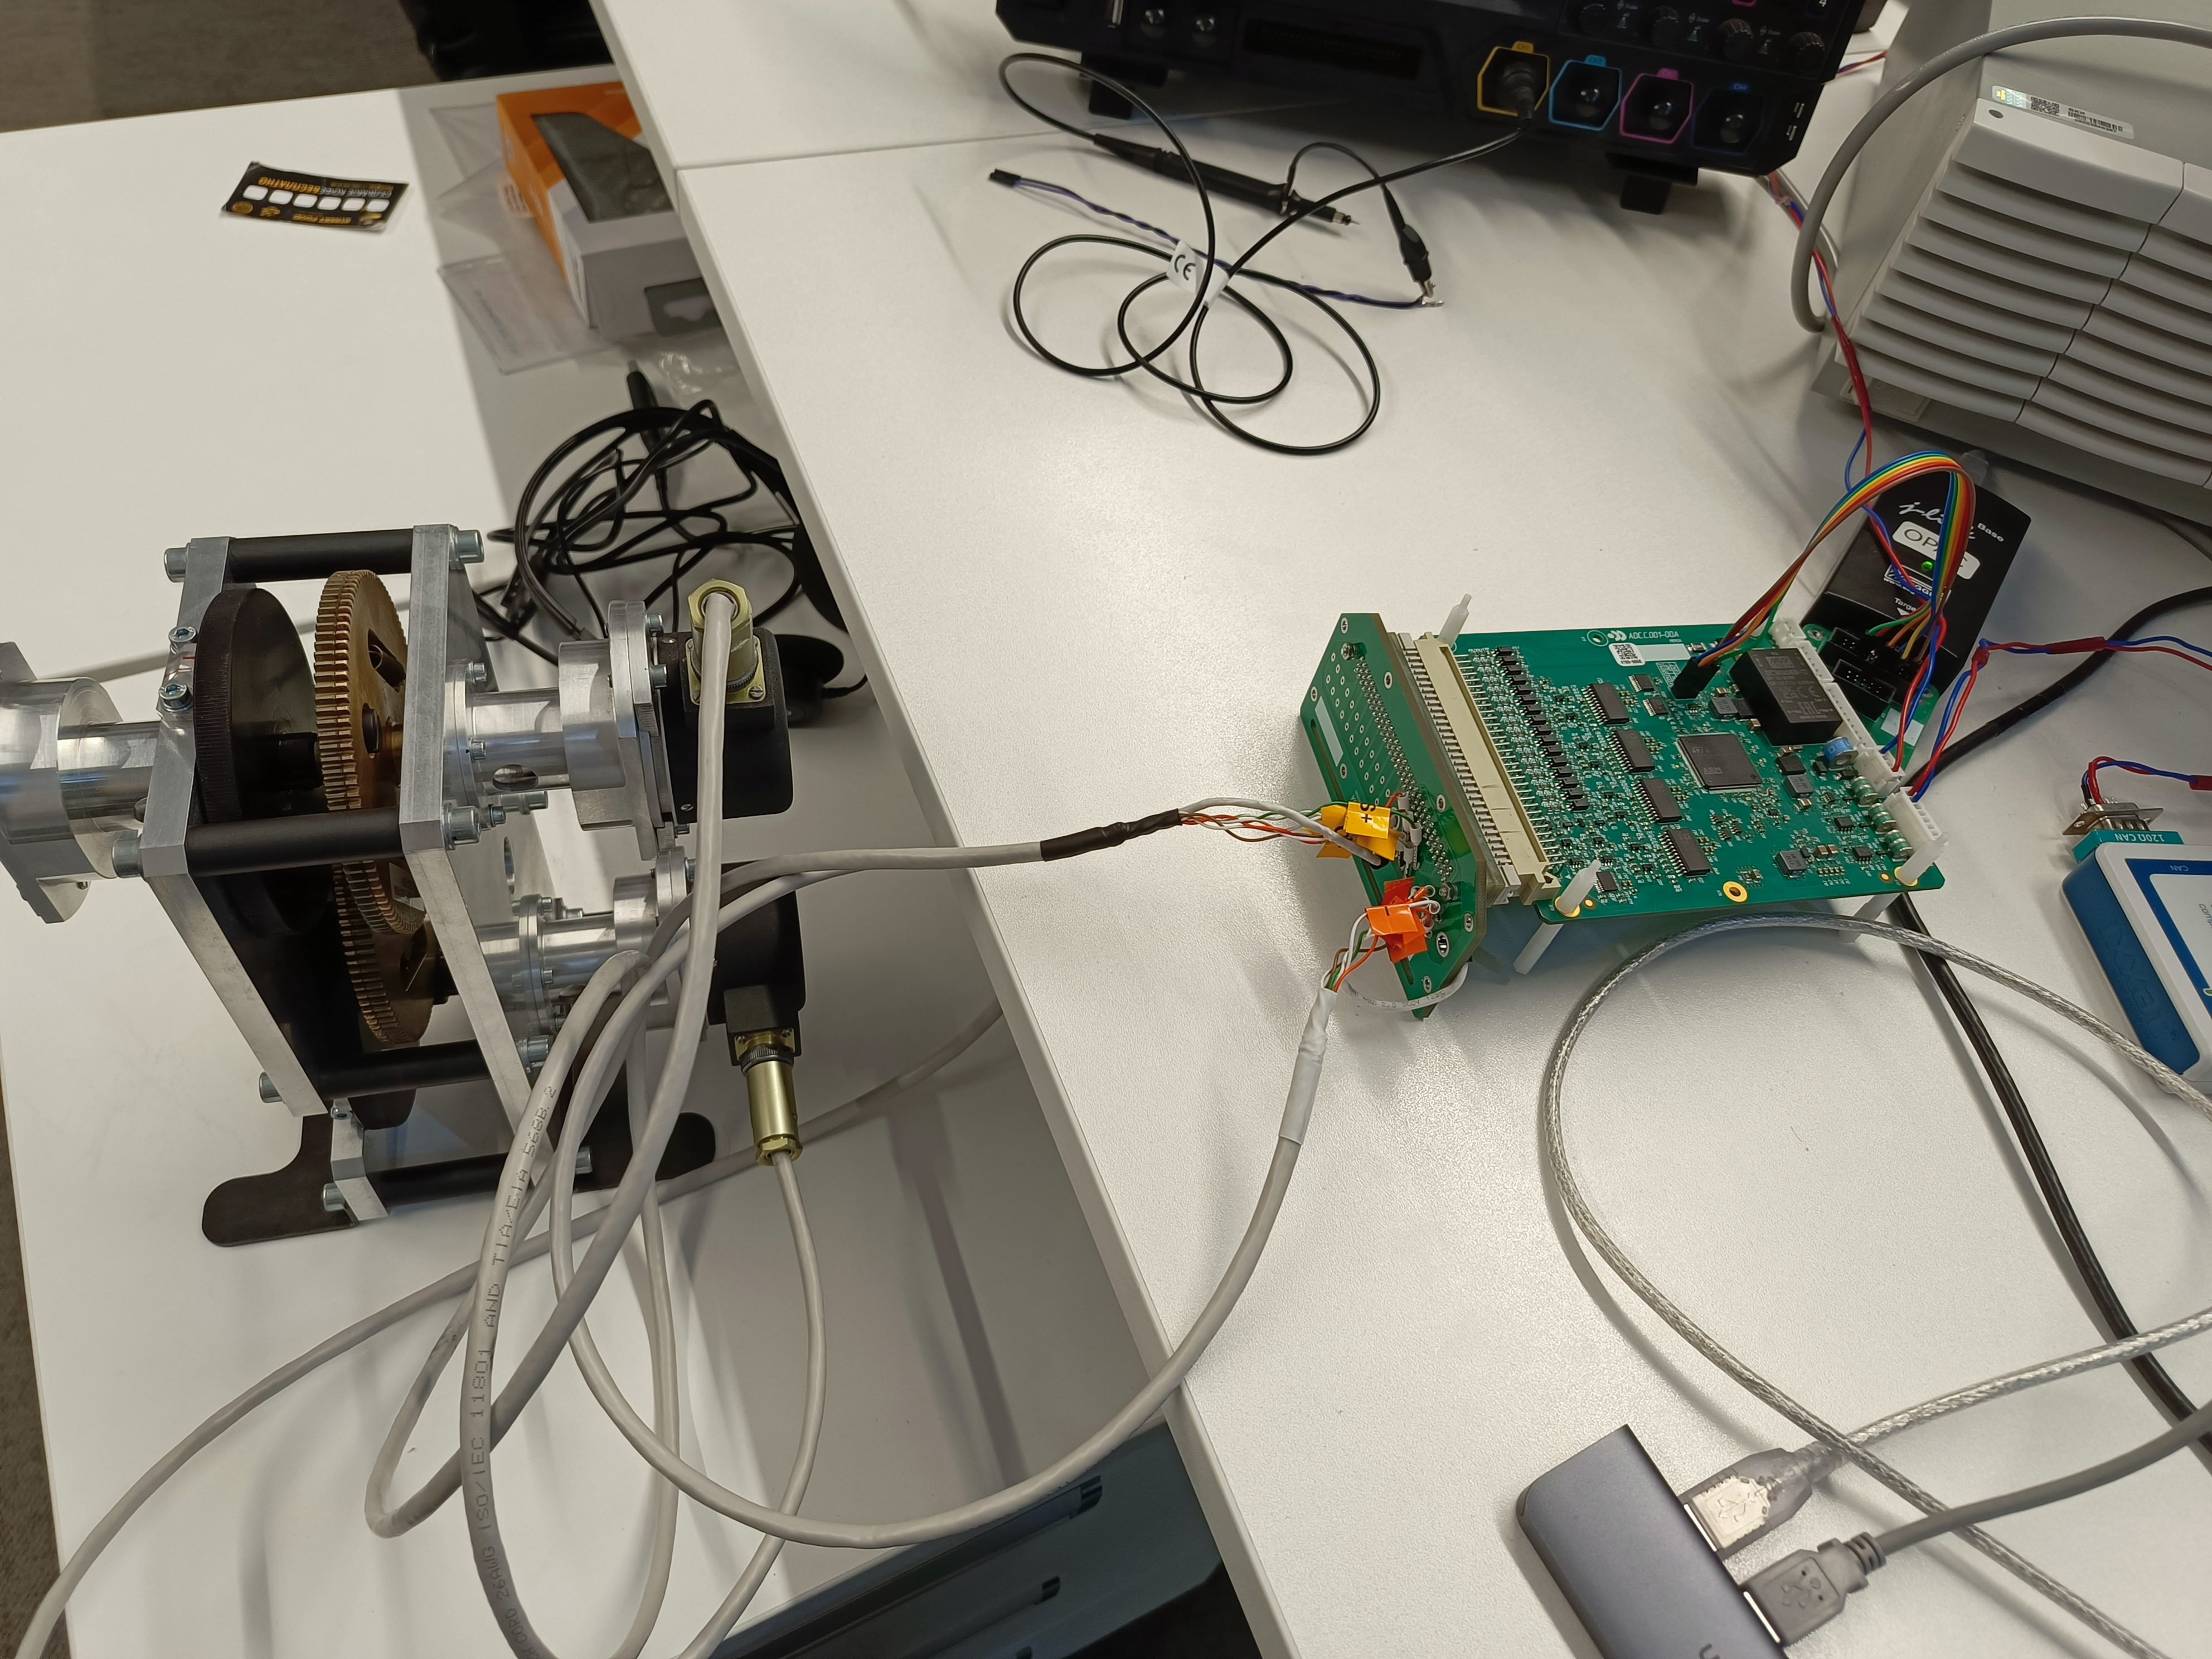
\includegraphics[width=\linewidth]{STND1.jpg} 
    \label{STND1}
  \end{subfigure}
  \hfill
  \begin{subfigure}[b]{0.35\textwidth}
    \centering
    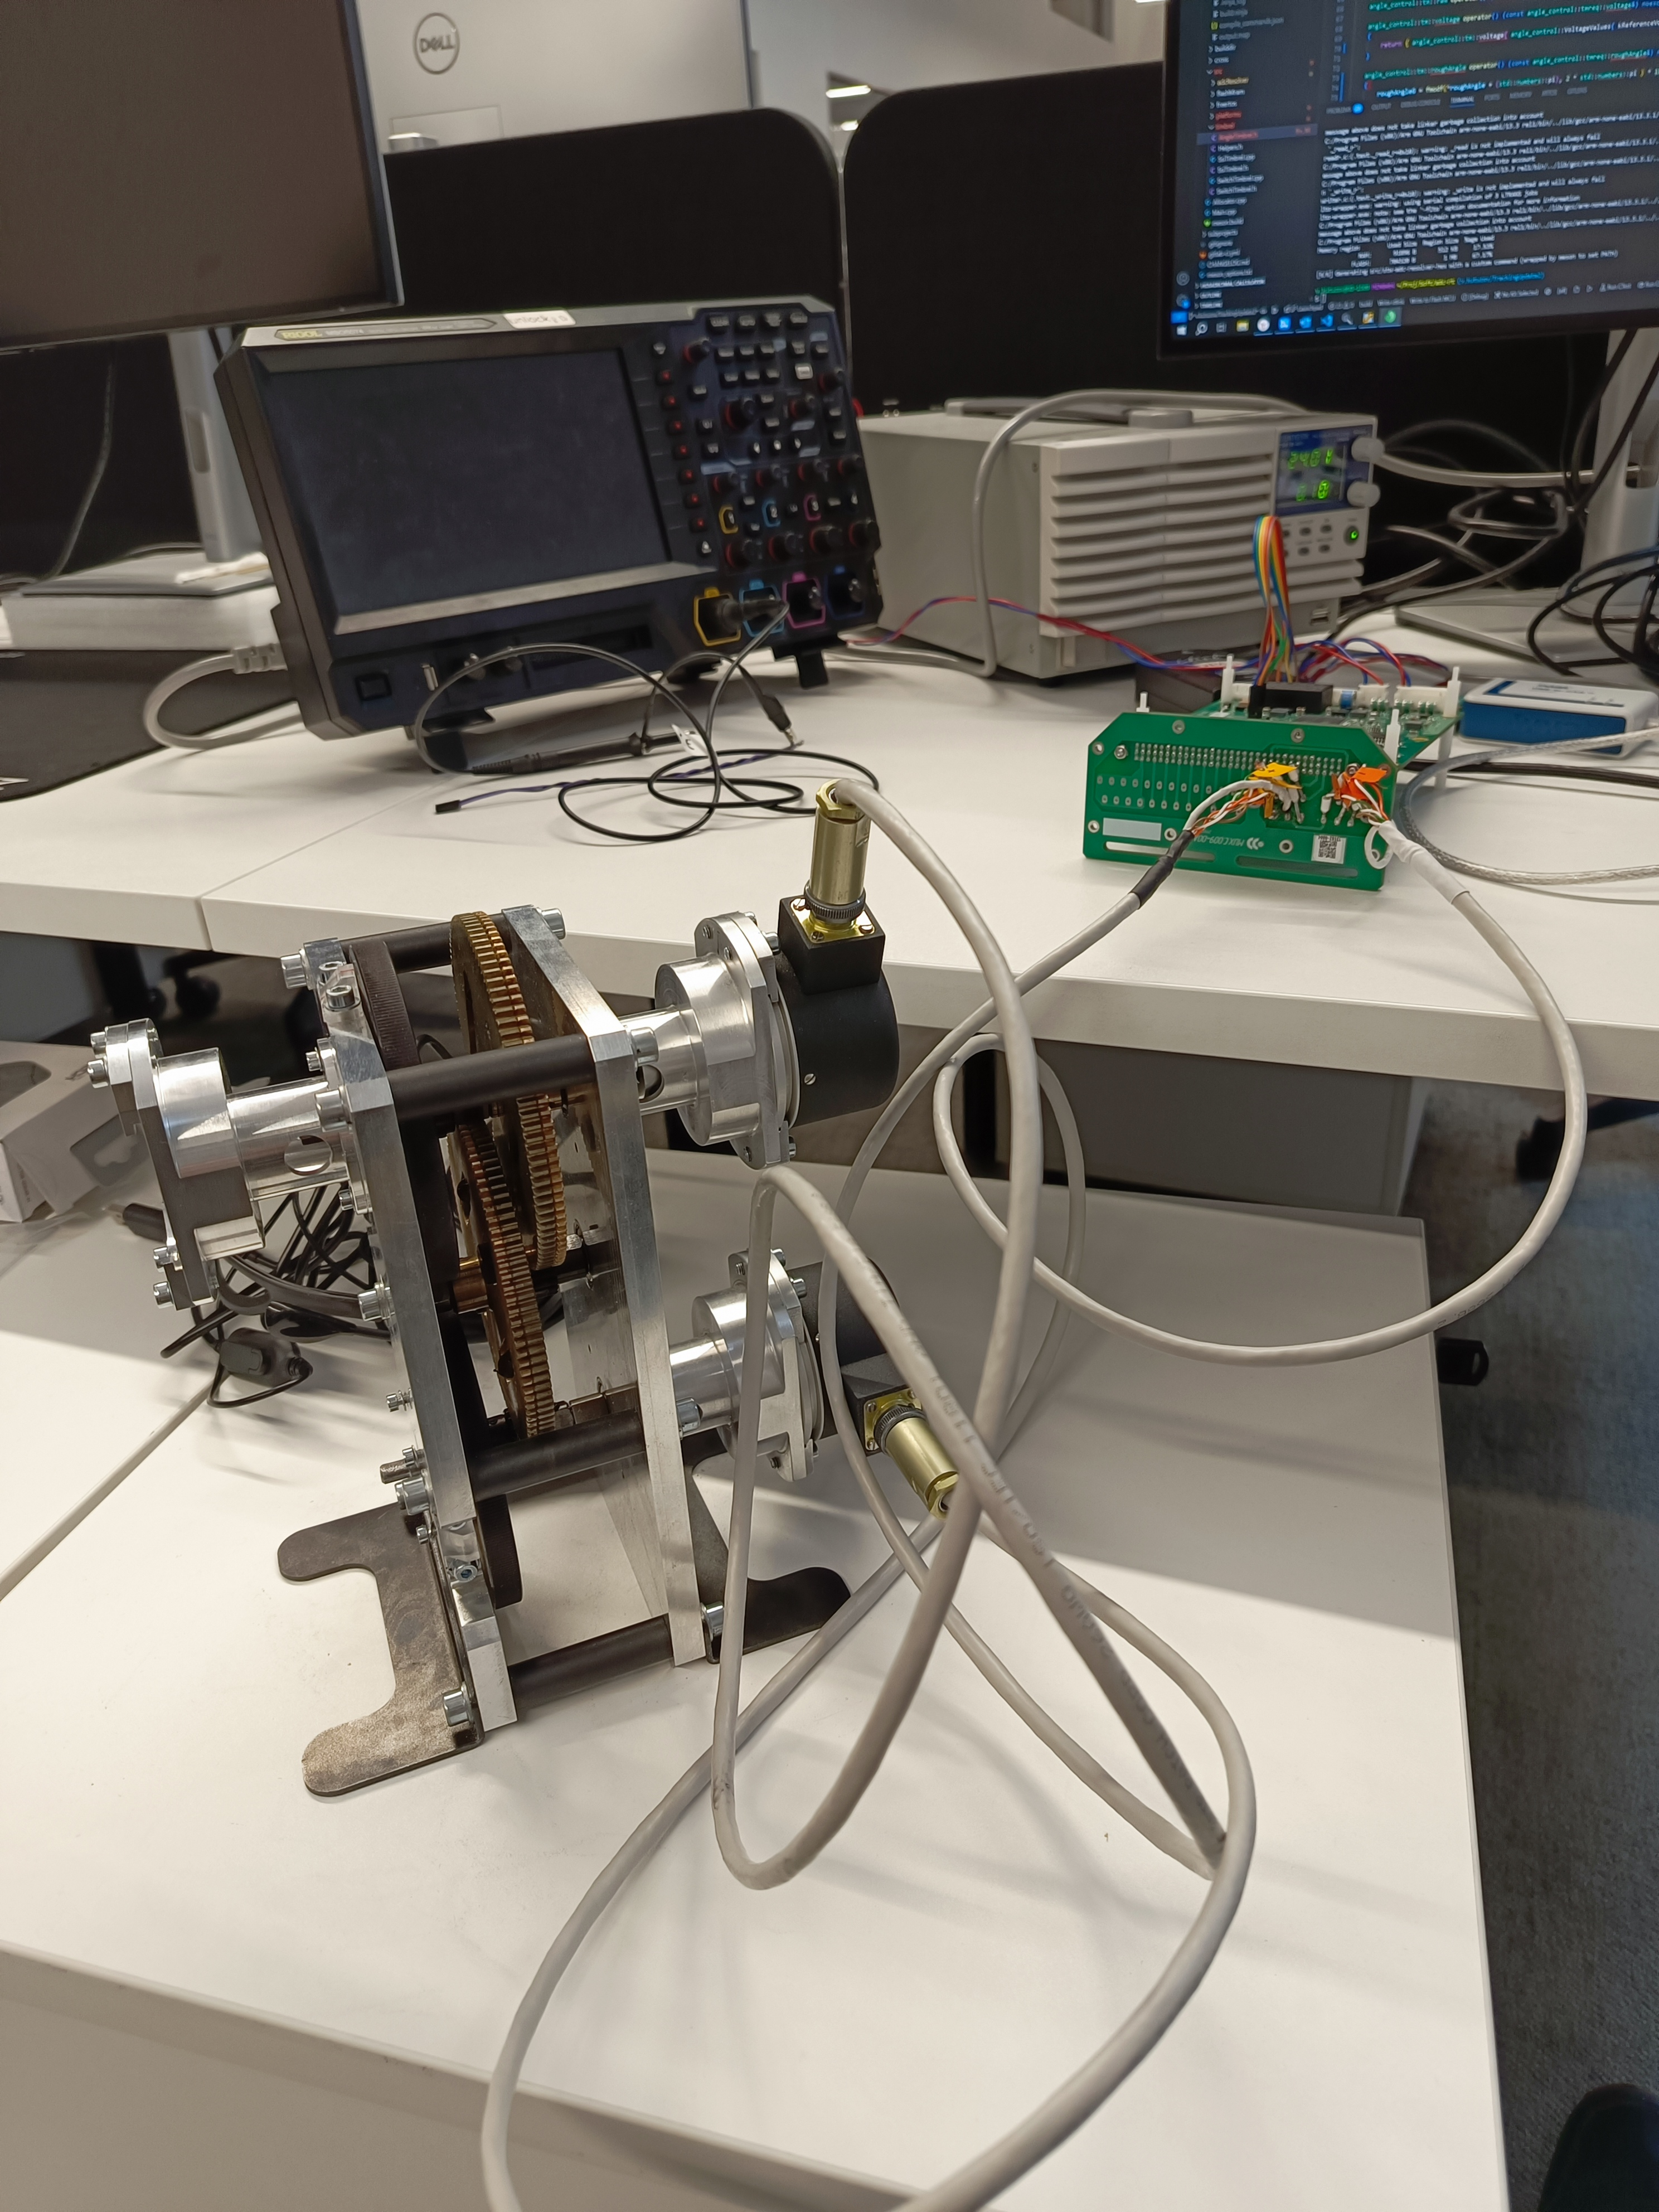
\includegraphics[width=\linewidth]{STND2.jpg} 
    \label{STND2}
  \end{subfigure}

  \caption{Тестировочный стенд}
  \label{STND} 
\end{figure}


\subsection{Характеристики сигнальных трактов}
\subsubsection{Входные воздействия}
На вход датчиков подаются синусоидальные сигналы, генерируемые по закону: %Добавить сюда фотографии с осц
\begin{equation}
    U_{in}(t) = A \cdot \sin(2\pi f t + \varphi_0), \quad 
\end{equation}
где $A$ = 7 В - амплитуда возбуждения, f = 10 кГц - частота.
Фазовый сдвиг $\varphi_0$ программно регулируется в диапазоне $0^\circ - 360^\circ$ с точностью $0,2^\circ$.

\subsubsection{Выходные сигналы}
Датчики формируют ортогональные сигналы, описываемые уравнениями:
\begin{align}
    U_{\sin} &= A \cdot \sin(k\theta) \\
    U_{\cos} &= A \cdot \cos(k\theta)
\end{align}
где $A = 7$В, $k=36$ - передаточное отношение, $\theta$ - измеряемый угол.

% Сигналы поступающие в датчик из схемы ЦАП с усилением \textbf{картинка синуса в датчик}
% Сигналы с датчика поступающие на АЦП \textbf{картинка косинусов с датчиков}


% \begin{figure}[!h]
%   \centering
%   \begin{subfigure}[b]{0.45\textwidth}
%     \centering
%     \includegraphics[width=\linewidth]{input_signal.png} 
%     \caption{Эталонные сигналы на входе датчиков}
%     \label{input_sig}
%   \end{subfigure}
%   \hfill
%   \begin{subfigure}[b]{0.45\textwidth}
%     \centering
%     \includegraphics[width=\linewidth]{output_signal.png} 
%     \caption{Выходные сигналы с датчиков}
%     \label{output_sig}
%   \end{subfigure}
%   \caption{Осциллограммы сигналов в контрольных точках}
% \end{figure}






